As introduced in Sec.~\ref{ssec:1_rl_bandit}, there exists other strategies than $\epsilon$-greedy ones, that balance between exploration and exploitation in Markov Reward Processes (MRP). Among them, we studied  UCB and TS ones. In this section we will equip the Q-learning agent introduced in Sec.~\ref{ssec:rl_cohql} to enchance the model-free calibration.

\begin{figure}[t!]
    \centering
    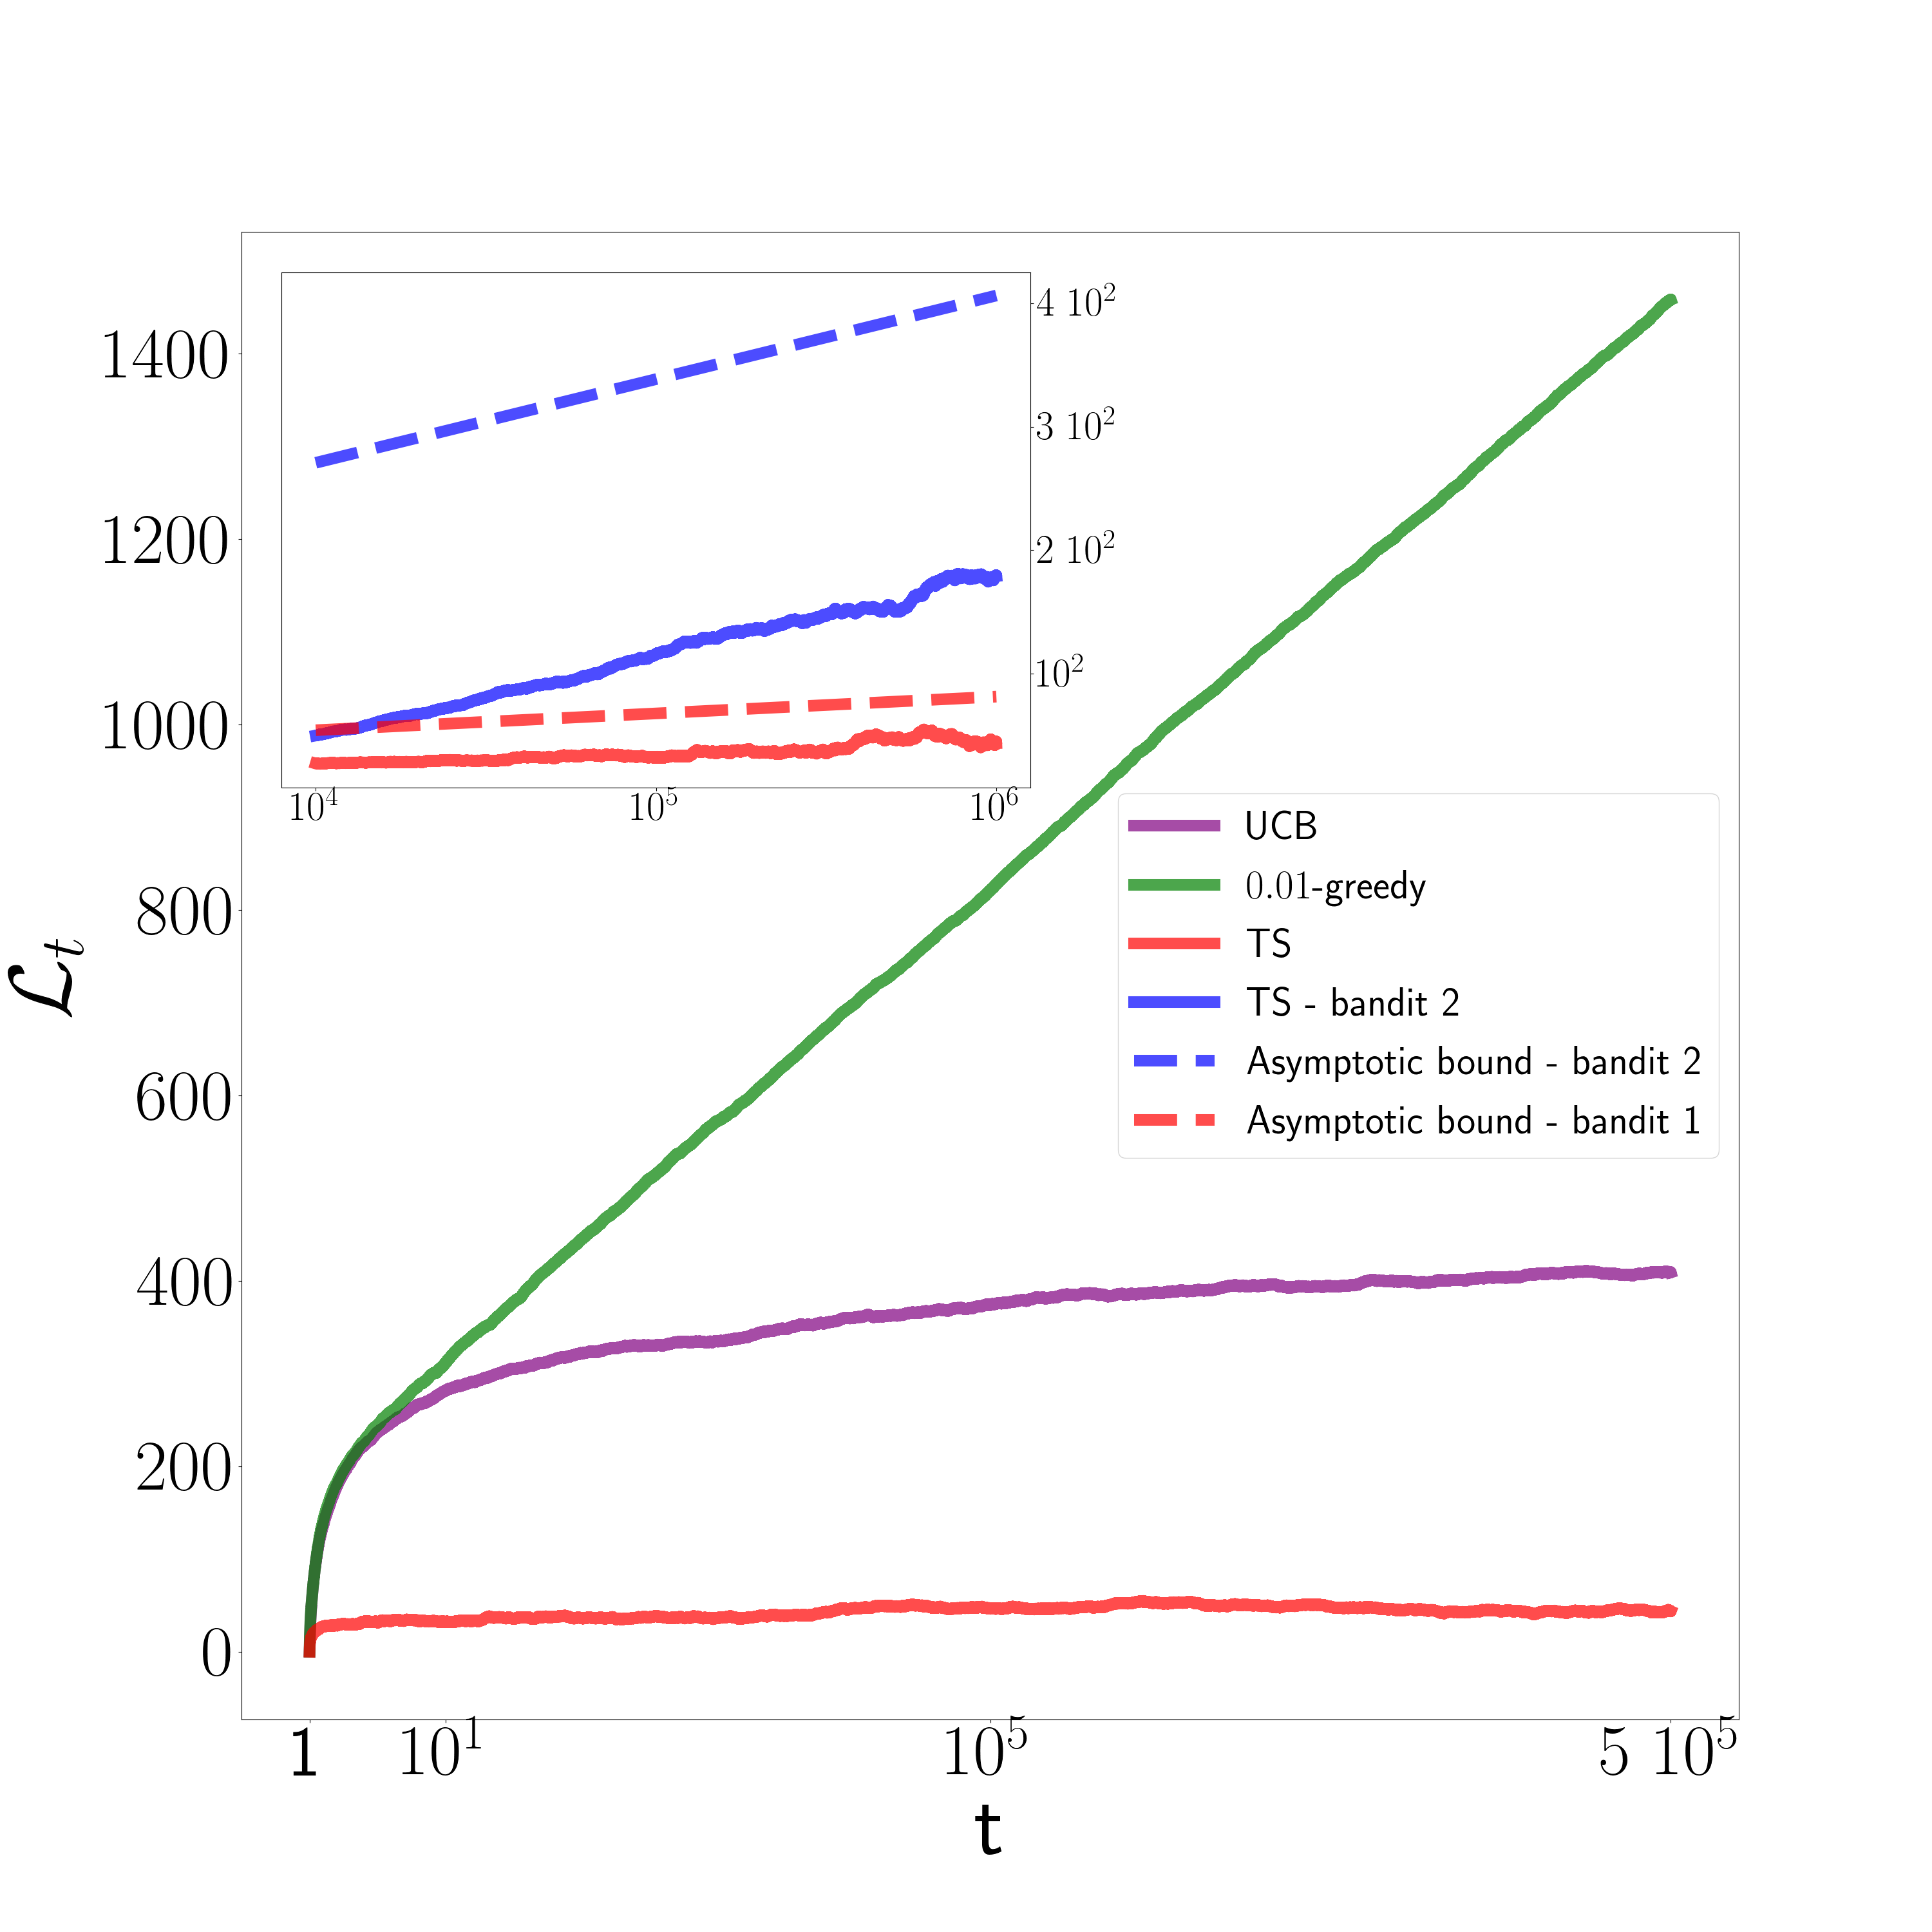
\includegraphics[width=0.9\textwidth]{Figures/1bandit/bandit_numerics_not_shifted.png}
    \caption{We show the evolution of the cumulative regret for three different policies: $\varepsilon$-greedy, UCB and TS in a bandit setting. The mean values considered are associated to success probabilities of Kennedy-like receivers, as introduced in Sec.~\ref{ssec:rlcoh_kennedyreceiver}. All curves are averaged  over $10^{3}$ agents. Specifically, they are Bernoulli distributions with different mean values, each associated to different configurations of a quantum receiver parametrized by a value $\beta$. For \textit{bandit problem 1}, we considered $\beta \in \{0, -\alpha, \beta^{*}\}$, with $\alpha = 0.4$ and $\beta^{*} = -0.74$.
    Furthermore, we compare the asymptotic behaviour of TS, studying \textit{bandit problem 2}, where $\beta \in \{-\alpha, \beta^{*}, -1.5 \alpha\}$, shown in the inset plot.}
    \label{fig:bandfig}
\end{figure}

\textit{Calibration of Kennedy-like receivers as a bandit-problem}. We will first consider the model-free calibration of a Kennedy-like receiver as a bandit-problem. To this end, we have numerically compared the performance of the three bandit policies discussed in Sec.~\ref{ssec:1_rl_bandit}. The bandit problem that we consider deals with three different Bernoulli distributions, each associated to a different value of a Kennedy receiver. At each episode the agent observes a reward of value either $0$ or $1$, obtained by guessing (max-likelihood) for the underlying phase of the coherent state by using the selected receiver. In Fig.~\ref{fig:bandfig} we show the expected regret $\mathcal{L}_t$ estimated out of several realizations of such 3-armed bandit problem. The figure shows that the cumulative regret scales linearly with time for the $\epsilon$-greedy strategy, while it has a logarithmic scaling for the UCB and TS strategies. The inset shows the cumulative regret as a function of $\log t$ together with the ultimate bound given by Lai-Robbins bound; we observe that sub-leading constants seem to still be relevant in such a bound, and that whereas assymptotic regime seems not to have been reached, the results are yet consistent with Eq.~\ref{eq:RLBOUND}.

We will now turn to use this strategies to improve the performance of the Q-learning agent considered previously. In particular, we will present two alternative strategies for the action exploration to be applied in the Q-learning algorithm.

The first strategy employs the standard Q-learning update rule for the estimate $\hat{Q}$, as described in Eq.~\eqref{eq:QLUPDATERULE}, but it uses UCB to determine the interaction policy at each time-step of each episode. Here, we recall that UCB choices the action according to an upper confidence bound of the form of Eq.~\ref{eq:ucbeq2}:
\begin{equation}
{\rm ucb}_{t}(a):=\hat{Q}(a)+\varepsilon(t) = \hat{Q}(a)+\sqrt{\frac{-\log \mathcal{P}(t)}{2 N_{t}(a)}} ,
\end{equation}
which represents an upper bound to the true value ${Q}(a)$ with a high probability $1-\mathcal{P}(t)$.

We have here chosen $\mathcal{P}(t)=t^{-4}$. This is implemented by keeping a count of the number of visits of each history-action couple up to the current episode $t$, i.e., $N_{t}(h_{\ell},a_{\ell})$, which is then used to compute an upper confidence bound, ${\rm ucb}_{t}(h_{\ell},a_{\ell})$ as in Eq.~\eqref{eq:ucbeq2}, for each action $a_{\ell}$ and history $h_{\ell}$. Finally, at time-step $\ell$ the agent chooses the greedy action with respect to the UCB, \textit{i.e.}, $a_{\ell}^{(t)}=\argmax{a}{\rm ucb}_{t}(h_{\ell},a)$.

The second strategy is instead based entirely on TS, considering each action conditioned on the past history as a bandit problem and rewarding each sequence of actions that led to a successful experiment. In detail, the agent keeps a beta-distribution, Eq.~\eqref{eq:betaDistro}, of the mean reward obtainable at each time-step $\ell$ from each action $a_{\ell}$ given each possible history $h_{\ell}$, i.e., $f_{t}(\bar{r}|h_{\ell},a_{\ell})$. In order to choose a new action at time-step $\ell$ given history $h_{\ell}$, the agent samples an expected reward $\bar{r} \sim f_{t}(\bar{r}|h_{\ell},a_{\ell})$ for each $a_{\ell}$
and selects the action with the largest sample $\bar{r}$.
At the end of the episode a reward is obtained as usual, and $f_{t}(\bar{r}|h_{\ell},a_{\ell})$ is updated in a Bayesian way for all the history-action couples visited at the episode. In this case, when computing $\Pt$, the best actions are chosen by going greedy with respect to their mean reward distribution $f_{t}(\bar{r}|h_{\ell},a_{\ell})$~\cite{Russo2018}.

In Fig.~\ref{fig:threemethods} we show the evolution of the two figures of merit $\Rt$, $\Pt$ for several agents trained using these two enhanced strategies, as well as for those based on the exp-greedy and $0.3$-greedy strategies, considered in Sec.~\ref{ssec:rlcoh_qlearning}, which had respectively the largest final $\Rt$ and $\Pt$ out of all the analyzed strategies.
We observe that UCB performs a thorough exploration of the action space and indeed it is able to attain a value of $\Pt$ close to that of $0.3$-greedy. This result comes at the price of a small $\Rt$ value, which nevertheless shows that UCB has better exploitation properties than $0.3$-greedy; in particular it has a strikingly larger slope than the latter at long times. As for TS, we observe that this strategy attains the best $\Rt$ values, surpassing exp-greedy at intermediate times. Moreover, TS also radically improves the values of $\Pt$ with respect to exp-greedy and it is even able to attain the performance of the other two strategies that favour exploration. Overall, it appears that for this particular problem setting, and the hyperparameters chosen for all three algorithms, TS provides the most profitable balance of exploration and exploitation.

\begin{figure}[t!]
    \centering
    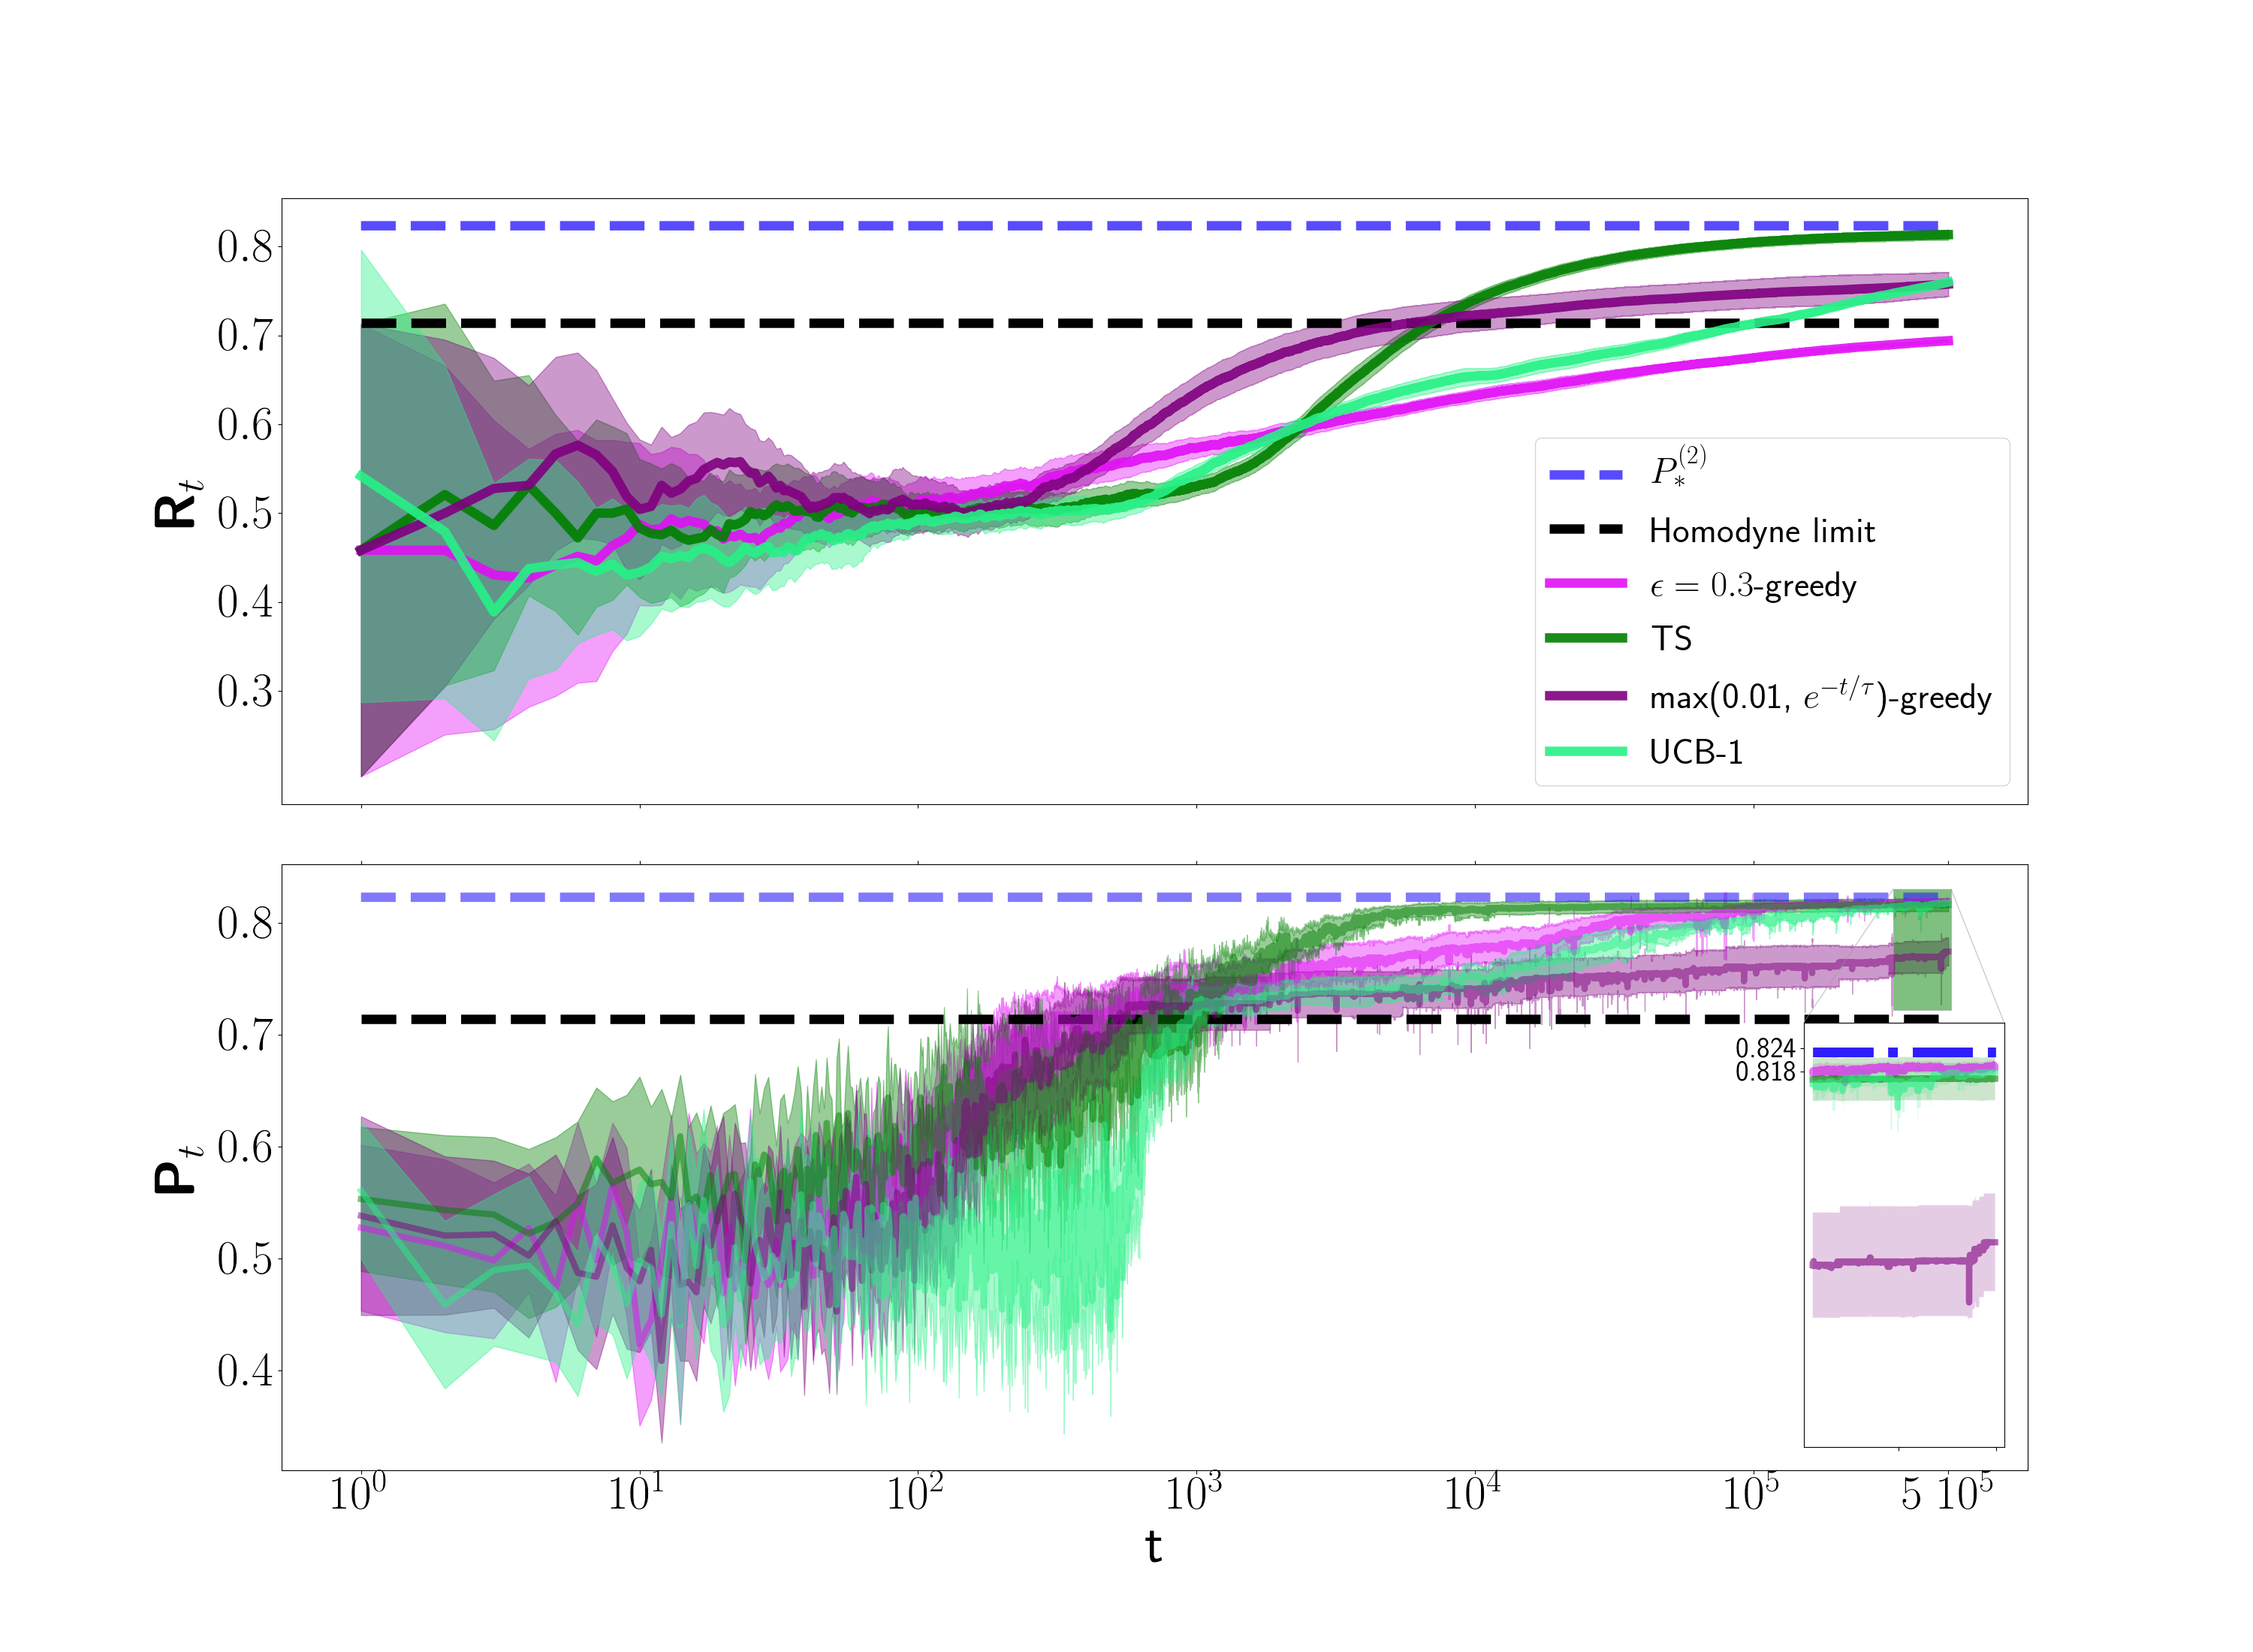
\includegraphics[width=1.\textwidth]{Figures/317/rev_enh-QLexp.png}
   \caption{We show the learning curves for the enhanced Q-learning agents via bandit methods. On the upper plot we despict $\Rt$, the agent's success rate per episode, whereas on the bottom plot we despict $\Pt$, the success probability of the agent's recommended actions at episode $t$, $\llaves{a_{\ell}^{(t)*}}$. Each of the learning curves is averaged over 48 agents; the amplitude was fixed to $\alpha = 0.4$.}
    \label{fig:threemethods}
\end{figure}

Overall, we observe that model-free Q-learning agents can readily learn to calibrate Dolinar-like receivers by beggining the learning task from the darkness, meaning that they complete ignore the setting at hand.

While such learning process is interesting on its own, we can now turn to non-ideal scenarios, which arguably is \textit{the} motivation of our setting. The reason for this is, on the one hand, that the presence of unknown quantum channels might non-trivially act on the signals, and thus the optimal configuration will differ to that one of the idealistic, noise-less case. On the other hand, we have assumed so far that there are no imperfections during the measurement process, an issue that is certainly present in experiments. For this reason, we will now turn to benchmark the performance of our model-free agents in a wide range of noisy scenarios.
